
% part  19
\section{Отмена deferred'ов\label{sec:part19}}


\subsection{Введение}


Twisted развивающийся проект и разработчики Twisted регулярно 
добавляют новые свойства и расширяют старые. В релиз Twisted 10.1.0, 
разработчики добавили новое свойство аннулирования в классе Deffered, 
которое мы собираемся изучить в этой главе.


Асинхронное программирование отделяет запросы от ответов, и 
таким образом генерирует новую возможность: между запросом  
результата и получением его обратно, вы можете решить больше 
не ждать. Рассмотрим поэтический прокси сервер из главы 14. 
Далее то, как работает прокси, по меньшей мере для первого 
запроса поэмы:

\begin{enumerate}
\item Приходит запрос поэмы.
\item Прокси соединяется с реальным сервером для получения поэмы.
\item После того, как вся поэма получена, отправляет ее запрашивающему клиенту.
\end{enumerate}


Все достаточно хорошо, но что, если клиент завис до получения 
поэмы? Может сначала клиент запросил одну поэму, потом передумал и 
решил, что ему надо другую. Теперь наш прокси застрял, скачивая первую 
поэму, и нашему медленному серверу понадобится некоторое время, чтобы 
ее передать. Лучше закрыть соединение и позволить медленному серверу 
опять ожидать нового запроса.

%Recall Figure 15, a diagram that shows the conceptual flow of control in a synchronous program. In that figure we see function calls going down, and exceptions going back up. If we wanted to cancel a synchronous function call (and this is just hypothetical) the flow control would go in the same direction as the function call, from high-level code to low-level code as in Figure 38:

Вспомним рисунок 15, на котором изображена диаграмма, 
которая показывает поток выполнения в синхронной программе. 
На этом рисунке мы видим низходящий поток вызовов функций и 
восходящий поток исключений. Если мы хотим аннулировать 
синхронный вызов фукнкции, направление потока выполнения 
было такое же как и в случае вызова функции, от высокоуровнего 
кодо до низкоуровнего, как это показано на рисунке \ref{fig:sync-cancel}.

% fig38
\begin{figure}[h]
\begin{center}
    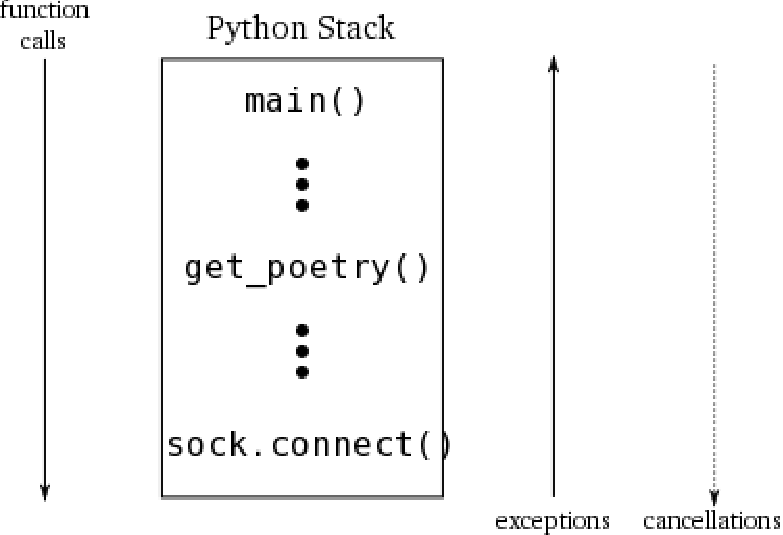
\includegraphics[width=0.5\textwidth]{images/sync-cancel.pdf}
    \caption{Поток выполнения в синхронной программе в случае гипотетического аннулирования\label{fig:sync-cancel}}
\end{center}
\end{figure}

Конечно же, в синхронной программе это невозможно, поскольку 
высокоуровневый код не может приостановиться до того 
момента, как низкоуровневые операции не завершатся, но с этого 
момента уже нечего аннулировать. Но в асинхронной программе 
высокоуровневый код получает контроль до того, как завершится 
низкоуровневый код, который может сгенерировать отмену низкоуровневого 
кода до момента его завершения.


В Twisted программе, низкоуровневый запрос реализуется 
объектом Deferred, про который вы можете думать как об 
обработчике невыполненной асинхронной операции. Обычный 
поток информации в deferred'е низходящий, от низкоуровневого 
кода до высокоуровнего, который сопоставляет поток возвращенной 
информации в синхронной программе. Начиная с Twisted 10.1.0, 
высокоуровневый код может отправить информацию обратно в 
другом направлении: он может сказать 
низкоуровневому коду, что не надо больше возобновляться. 
Посмотрите на рисунок \ref{fig:deferred-cancel}.

% fig39
\begin{figure}[h]  
\begin{center}
    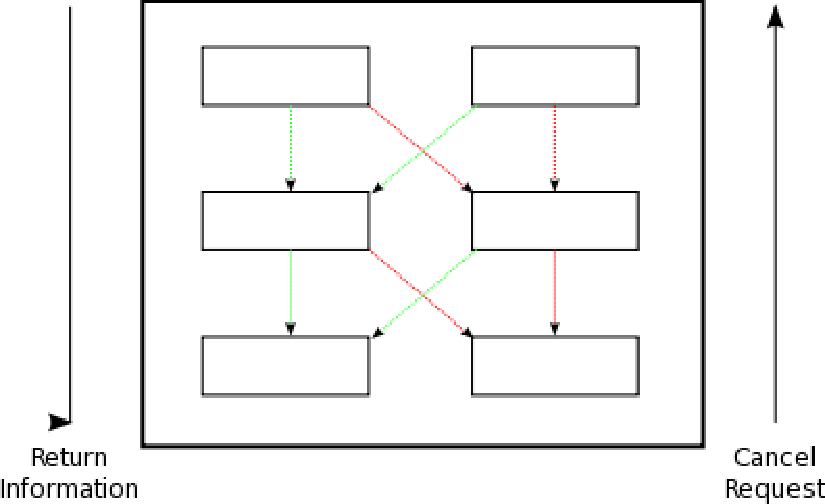
\includegraphics[width=0.5\textwidth]{images/deferred-cancel.pdf}
    \caption{Информационный поток в deferred'е, включая аннулирование\label{fig:deferred-cancel}}
\end{center}
\end{figure}


\subsection{Аннулирующиеся deferred'ы}

Давайте посмотрим на несколько примеров программ, чтобы увидеть 
как в действительности работает аннулирование deferred'ов. Чтобы запускать 
примеры из этой главы, нужно иметь 
\href{http://twistedmatrix.com/trac/wiki/Downloads}{Twisted версии 10.1.0 или выше}.  
Рассмотрим \href{http://github.com/jdavisp3/twisted-intro/blob/master/deferred-cancel/defer-cancel-1.py#L1}{deferred-cancel/defer-cancel-1.py}:

\begin{scriptsize}\begin{verbatim}
from twisted.internet import defer

def callback(res):
    print 'callback got:', res

d = defer.Deferred()
d.addCallback(callback)
d.cancel()
print 'done'
\end{verbatim}\end{scriptsize}


С новым свойством аннулирования, класс Deferred имеет новый 
метод с названием cancel. В примере создается deferred, 
добавляется callback и затем вызывается функция cancel без 
активизации deferred'а.  Далее вывод:

\begin{scriptsize}\begin{verbatim}
done
Unhandled error in Deferred:
Traceback (most recent call last):
Failure: twisted.internet.defer.CancelledError:
\end{verbatim}\end{scriptsize}


Таким образом аннулирование deferred'а вызывает запуск 
цепочки errback, и обычный callback никогда не вызывается. 
Заметим, что ошибка типа twisted.internet.defer.CancelledError, 
является пользовательским Exception, означающим, что deferred 
был аннулирован. Давайте добавим errback в 
\href{http://github.com/jdavisp3/twisted-intro/blob/master/deferred-cancel/defer-cancel-2.py#L1}{deferred-cancel/defer-cancel-2.py}:

\begin{scriptsize}\begin{verbatim}
from twisted.internet import defer

def callback(res):
    print 'callback got:', res

def errback(err):
    print 'errback got:', err

d = defer.Deferred()
d.addCallbacks(callback, errback)
d.cancel()
print 'done'
\end{verbatim}\end{scriptsize}

Теперь мы получаем следующий вывод:

\begin{scriptsize}\begin{verbatim}
errback got: [Failure instance: Traceback (failure with no frames): 
<class 'twisted.internet.defer.CancelledError'>:]
done
\end{verbatim}\end{scriptsize}

То есть мы можем поймать аннулирование в errback'е подобно тому, как 
возникновление обычной ошибки в deferred'е.


Давайте попытаемся активизировать deferred и 
затем его дективизируем так, как в примере 
\href{http://github.com/jdavisp3/twisted-intro/blob/master/deferred-cancel/defer-cancel-3.py#L1}{deferred-cancel/defer-cancel-3.py}:


\begin{scriptsize}\begin{verbatim}
from twisted.internet import defer

def callback(res):
    print 'callback got:', res

def errback(err):
    print 'errback got:', err

d = defer.Deferred()
d.addCallbacks(callback, errback)
d.callback('result')
d.cancel()
print 'done'
\end{verbatim}\end{scriptsize}


Здесь мы активизировали deferred обычным образом 
методом callback и затем его деактивизировали. Далее вывод:

\begin{scriptsize}\begin{verbatim}
callback got: result
done
\end{verbatim}\end{scriptsize}


Наш callback был вызван (так как мы и ожидали), и 
программа нормально завершилась, так будто cancel  
никогда не вызывался. Таким образом, аннулирование уже 
активизиврованного deferred'а не оказывает влияния.


Что если мы активизируем deferred после его 
аннулирования так, как это сделано в 
\href{http://github.com/jdavisp3/twisted-intro/blob/master/deferred-cancel/defer-cancel-4.py#L1}{deferred-cancel/defer-cancel-4.py}?


\begin{scriptsize}\begin{verbatim}
from twisted.internet import defer

def callback(res):
    print 'callback got:', res

def errback(err):
    print 'errback got:', err

d = defer.Deferred()
d.addCallbacks(callback, errback)
d.cancel()
d.callback('result')
print 'done'
\end{verbatim}\end{scriptsize}

В этом случае мы получаем следующий вывод:

\begin{scriptsize}\begin{verbatim}
errback got: [Failure instance: Traceback (failure with no frames): 
<class 'twisted.internet.defer.CancelledError'>:]
done
\end{verbatim}\end{scriptsize}


Та же выдача, что и во втором примере, где мы никогда не 
активизировали deferred. Но почему вызов d.callback('result') 
не спровоцировал ошибку, из предположения, что deferred не может 
быть активизирован более одного раза и из предположения, что 
цепочка errback явно была запущена?


Посмотрим снова на рисунок \ref{fig:deferred-cancel}. Активизация 
deferred'а с результатом или ошибкой -  низкоуровневая задача, 
в то время как сброс deferred'а - действие, производимое 
высокоуровневым кодом. Активизация deferred'а означает ``Вот Ваш результат'', 
в то время как сброс deferred'а означает ``Я больше этого не хочу''. 
Запомните, что сброс - новое свойство, поэтому большая часть Twisted 
кода не написана для управления операциями сброса. Но разработчики 
Twisted сделали возможным для нас сбрасывать любые deferred's, 
даже, если имеющийся код был написан до Twisted 10.1.0.


Для того, чтобы сделать это возможным, метод cancel 
в дейcтвительности делает две вещи:

\begin{enumerate}
\item Скажи объекту Deferred, что ты не хочешь получить результат, если он 
    еще не сформировался (например, deferred еще не был активизирован), и 
    проигнорируй любые последовательные вызовы callback и errback.

\item Опционально: скажи низкоуровневому коду, который производит результат, 
    принять любые меры, требующиеся для отмены операции.
\end{enumerate}


Для совместимости со старыми версиями Twisted 
отмененный deferred все равно активизируется, 
шаг 1 гарантирует, что наша программа не будет 
блокироваться, если  мы отменим deferred из более 
старой версии библиотеки.


Это означает, что мы всегда можем отменить deferred, и мы 
будем уверены, что не получим результат, если он еще не 
прибыл (даже, если прибудет позже). Но отмена deferred'а может 
в действительности не отменить асинхронную операцию. Сброс 
асинхронной опрации требует контекстно-специфичного действия. 
вам нужно закрыть сетевое соединение, откатить транзакцию к 
базе данных, убить подпроцесс и т. д. Посколько deferred - 
просто callback организатор общего назначения, как он 
узнает, что нужно выполнить какое-то специфичное дейтсвие при 
его отмене? Или, иначе, как он мог бы перенаправить запрос 
на отмену низкоуровневому коду, который создал и возвратил 
deferred? Ответ - с помощью callback'а. 

    
\subsection{Действительно отмененные Deferred'ы}

Взглянем на 
\href{http://github.com/jdavisp3/twisted-intro/blob/master/deferred-cancel/defer-cancel-5.py#L1}{deferred-cancel/defer-cancel-5.py}:

\begin{scriptsize}\begin{verbatim}
from twisted.internet import defer

def canceller(d):
    print "I need to cancel this deferred:", d

def callback(res):
    print 'callback got:', res

def errback(err):
    print 'errback got:', err

d = defer.Deferred(canceller) # created by lower-level code
d.addCallbacks(callback, errback) # added by higher-level code
d.cancel()
print 'done'
\end{verbatim}\end{scriptsize}


Этот код в основном подобен второму примеру, 
за тем лишь исключением, что существует третий 
callback (canceller), который подставляется в Deferred, 
когда мы его создаем, а не после создания. Этот callback 
несет ответсвенность за выполнение контекстно-специфичных 
действий, требующихся для прерывания асинхронной операции (только, 
если deferred действительно отменяется, конечно же). callback 
canceller - необходимая часть низкоуровневого кода, 
который возвращает deferred, это не высокоуровневый код, 
который получает deferred и добавляет свои callback'и и errback'и.


Запущенный пример производит вывод:

\begin{scriptsize}\begin{verbatim}
I need to cancel this deferred: <Deferred at 0xb7669d2cL>
errback got: [Failure instance: Traceback (failure with no frames): 
<class 'twisted.internet.defer.CancelledError'>:]
done
\end{verbatim}\end{scriptsize}


Как вы видите, callback canceller вызывается deferred'ом при
отмене. В эту функцию помещаются любые действия, которые 
нужны для отмены асинхронной операции. Заметим, что canceller 
вызывается до того, как активизируется цепочка errback. Фактически, 
мы можем выбрать активизировать самим deferred в этом месте с 
любым результатом или ошибкой на наш выбор (таким образом, 
упреждая ошибку CancelledError). Обе возможности проиллюстрированы 
в \href{http://github.com/jdavisp3/twisted-intro/blob/master/deferred-cancel/defer-cancel-6.py#L1}{deferred-cancel/defer-cancel-6.py} и 
\href{http://github.com/jdavisp3/twisted-intro/blob/master/deferred-cancel/defer-cancel-7.py#L1}{deferred-cancel/defer-cancel-7.py}.


Давайте сделаем еще один простой тест, до того как 
мы запустим reactor. Создадим deferred c callback'ом 
canceller, активизируем его и отменим. Пример кода в 
\href{http://github.com/jdavisp3/twisted-intro/blob/master/deferred-cancel/defer-cancel-8.py#L1}{deferred-cancel/defer-cancel-8.py}. Изучая вывод этого скрипта, мы можем 
понять, что отмена deferred'а после его активизации не 
вызывает callback функцию canceller. И это то, что мы и ожидали, 
поскольку нечего отменять.


Примеры, на которые мы смотрели, в действительности 
не содержат асинхронных операций. Давайте сделаем 
простую программу, которая вызывает одну асинхронную 
операцию, затем мы выясним, как сделать возможность 
отменять эту операцию. Рассмотрим код 
\href{http://github.com/jdavisp3/twisted-intro/blob/master/deferred-cancel/defer-cancel-9.py#L1}{deferred-cancel/defer-cancel-9.py}:

\begin{scriptsize}\begin{verbatim}
from twisted.internet.defer import Deferred

def send_poem(d):
    print 'Sending poem'
    d.callback('Once upon a midnight dreary')

def get_poem():
    """Return a poem 5 seconds later."""
    from twisted.internet import reactor
    d = Deferred()
    reactor.callLater(5, send_poem, d)
    return d

def got_poem(poem):
    print 'I got a poem:', poem

def poem_error(err):
    print 'get_poem failed:', err

def main():
    from twisted.internet import reactor
    reactor.callLater(10, reactor.stop) # stop the reactor in 10 seconds

    d = get_poem()
    d.addCallbacks(got_poem, poem_error)

    reactor.run()

main()
\end{verbatim}\end{scriptsize}


Этот пример включает функцию get\_poem, которая использует метод 
rector'а callLater, для того, чтобы возвратить поэму через 5 секунд 
после вызова get\_poem. Функция main вызывает get\_poem, добавляет 
пару callback/errback, затем запускает reactor. Мы также останавливаем 
reactor через 10 секунд (снова используя callLater). Обычно мы бы 
делали это добавлением callback'а в deferred, но позже мы увидим, 
почему мы делаем это таким способом.


Запуск примера производит следующий вывод (после соответсвующей задержки):

 \begin{scriptsize}\begin{verbatim}
Sending poem
I got a poem: Once upon a midnight dreary
\end{verbatim}\end{scriptsize}

После 10 секунд наша маленькая программа завершается. Теперь 
давайте попробуем отменить deferred до того, как отправится поэма. 
Мы добавим небольшой код для отмены deferred'а через 2 минуты:


\begin{scriptsize}\begin{verbatim}
    reactor.callLater(2, d.cancel) # cancel after 2 seconds
\end{verbatim}\end{scriptsize}

Исходники нового примера находятся в 
\href{http://github.com/jdavisp3/twisted-intro/blob/master/deferred-cancel/defer-cancel-10.py#L1}{deferred-cancel/defer-cancel-10.py}, при запуске получаем вывод:

\begin{scriptsize}\begin{verbatim}
get_poem failed: [Failure instance: Traceback (failure with no frames): 
<class 'twisted.internet.defer.CancelledError'>:]
Sending poem
\end{verbatim}\end{scriptsize}


Этот пример ясно иллюстрирует, что отмена deferred'f 
не обязательно отменяет асинхронный вызов. После 2 
секунд мы увидим вывод нашего errback'а, печатающего 
CancelledError, как мы и ожидали. Затем, после 5 секунд, 
мы увидим вывод из send\_poem (но callback в deferred'е не 
будет активизироваться).


В этом месте , мы в той же ситуации, что и в примере 
\href{http://github.com/jdavisp3/twisted-intro/blob/master/deferred-cancel/defer-cancel-4.py#L1}{deferred-cancel/defer-cancel-4.py}. Отмена deferred'а вызывает то, что окончательный 
результат игнорируется, но не вызывает прерывания операции. Как мы 
изучили выше, чтобы сделать реальную возможность 
отмены deferred'а, мы должны добавить отменяющий callback при 
создании deferred'а.


Что должен делать новый callback? Посмотрим в 
\href{http://twistedmatrix.com/trac/browser/tags/releases/twisted-10.1.0/twisted/internet/interfaces.py#L556}{документацию} для 
метода callLater. Возвращаемое значение callLater - еще 
один объект, реализующий IDelayedCall, с методом 
cancel, который мы можем использовать для того, чтобы 
предотвратить выполнение отложенных вызовов.


Обновленный код находится в \href{http://github.com/jdavisp3/twisted-intro/blob/master/deferred-cancel/defer-cancel-11.py#L1}{deferred-cancel/defer-cancel-11.py}. Значимые изменения находятся в 
функции get\_poem:

\begin{scriptsize}\begin{verbatim}
def get_poem():
    """Return a poem 5 seconds later."""

    def canceler(d):
        # They don't want the poem anymore, so cancel the delayed call
        delayed_call.cancel()

        # At this point we have three choices:
        #   1. Do nothing, and the deferred will fire the errback
        #      chain with CancelledError.
        #   2. Fire the errback chain with a different error.
        #   3. Fire the callback chain with an alternative result.

    d = Deferred(canceler)

    from twisted.internet import reactor
    delayed_call = reactor.callLater(5, send_poem, d)

    return d
\end{verbatim}\end{scriptsize}


В этой новой версии, мы сохраняем возвращаемое значение 
фукции callLater, поэтому мы можем использовать его в 
нашем cancel callback'е. Единственное, что наш callback 
должен сделать - вызвать delayed\_call.cancel(). Как мы обсудили 
ранее, мы могли бы также выбрать активизацию deferred'а. 
Последняя версия нашего примера выводит:

\begin{scriptsize}\begin{verbatim}
get_poem failed: [Failure instance: Traceback (failure with no frames): 
<class 'twisted.internet.defer.CancelledError'>:]
\end{verbatim}\end{scriptsize}


Как видите, deferred отменился и асинхронная 
операция была дейтсвительно прервана (например, мы больше 
не видим вывод функции send\_poem).

 
\subsection{Поэтический прокси 3.0}

Как мы обсуждали во введении, поэтический прокси сервер - 
хороший кандидат для реализации отмены, так как это 
позволяет нам прерывать скачивание поэмы, если так получилась, 
что она никому не нужна (например, клиент закрывает соединение 
до того, как мы отправили поэму). Версия прокси 3.0 находится 
\href{http://github.com/jdavisp3/twisted-intro/blob/master/twisted-server-4/poetry-proxy.py#L1}{twisted-server-4/poetry-proxy.py} и реализует отмену deferred'ов. Первое изменение в 
\href{http://github.com/jdavisp3/twisted-intro/blob/master/twisted-server-4/poetry-proxy.py#L52}{PoetryProxyProtocol}:

\begin{scriptsize}\begin{verbatim}
class PoetryProxyProtocol(Protocol):

    def connectionMade(self):
        self.deferred = self.factory.service.get_poem()
        self.deferred.addCallback(self.transport.write)
        self.deferred.addBoth(lambda r: self.transport.loseConnection())

    def connectionLost(self, reason):
        if self.deferred is not None:
            deferred, self.deferred = self.deferred, None
            deferred.cancel() # cancel the deferred if it hasn't fired
\end{verbatim}\end{scriptsize} 

Вы можете сравнить со 
\href{http://github.com/jdavisp3/twisted-intro/blob/master/twisted-server-2/poetry-proxy.py#L52}{старой версией}. Два основных изменения:
\begin{enumerate}
\item Сохраняет deferred, который мы получили из get\_poem так, чтобы 
    мы могли позже его отменить, если понадобится.

\item Отменяет deferred при закрытии соединения. Заметим, что 
    deferred'ы также отменяются, после того, как мы действительно получили 
    поэму, но, как мы поняли из примеров, отмена активизированного deferred'а 
    не оказывает никакого воздейстсвия.
\end{enumerate}


Теперь нам нужно убедиться в том, что отмена deferred'а 
действительно прерывает скачивание поэмы. Для этого мы должны 
изменить \href{http://github.com/jdavisp3/twisted-intro/blob/master/twisted-server-4/poetry-proxy.py#L105}{ProxyService}: 

\begin{scriptsize}\begin{verbatim}
class ProxyService(object):

    poem = None # the cached poem

    def __init__(self, host, port):
        self.host = host
        self.port = port

    def get_poem(self):
        if self.poem is not None:
            print 'Using cached poem.'
            # return an already-fired deferred
            return succeed(self.poem)

        def canceler(d):
            print 'Canceling poem download.'
            factory.deferred = None
            connector.disconnect()

        print 'Fetching poem from server.'
        deferred = Deferred(canceler)
        deferred.addCallback(self.set_poem)
        factory = PoetryClientFactory(deferred)
        from twisted.internet import reactor
        connector = reactor.connectTCP(self.host, self.port, factory)
        return factory.deferred

    def set_poem(self, poem):
        self.poem = poem
        return poem
\end{verbatim}\end{scriptsize}

Можно сравнить со 
\href{http://github.com/jdavisp3/twisted-intro/blob/master/twisted-server-2/poetry-proxy.py#100}{старой версией}. 
В этом классе несколько больше изменений:

\begin{enumerate}

\item Мы сохраняем возвращаемое значение из reactor.connectTCP, 
    объект IConnector. Мы можем использовать метод для сохраненного 
    объекта для закрытия соединения.

\item Мы создаем deferred с callback'ом canceler. Этот 
    callback является замыканием, которое использует 
    connector для закрытия соединения. Но сначала атрибут 
    factory.deferred выставляется в None. Иначе, factory 
    может активизировать errback deferred'а с ошибкой ``закрытое 
    соединение'' до того, как deferred сам активизирует errback  
    с ошибкой CancelledError. После того, как deferred 
    был отменен, иметь активизированный deferred c CancelledError, 
    кажется более явным.

\end{enumerate}


вы можете заметить, что теперь мы создаем deferred в 
ProxyService вместо PoetryClientFactory. Поскольку 
callback canceler нуждается в доступе к объекту IConnector, 
ProxyService - наиболее удобное место для создания 
deferred'а.


Также, как в одном из наших ранних примерах, наш callback 
canceler реализован как замыкание. Замыкания кажутся очень 
полезными при реализации отменяющих callback'ов!


Давайте испытаем наш проки сервер. Сначала запустим медленный сервер. 
Он должен быть медленным для того, чтобы мы действительно имели 
время отменить:

\begin{scriptsize}\begin{verbatim}
python blocking-server/slowpoetry.py --port 10001 poetry/fascination.txt
\end{verbatim}\end{scriptsize}

Теперь мы можем запустить наш прокси (потребуется Twisted 10.1.0 или выше):

\begin{scriptsize}\begin{verbatim}
python twisted-server-4/poetry-proxy.py --port 10000 10001
\end{verbatim}\end{scriptsize}

Теперь мы можем начать скачивать поэму из сервера, используя любой 
клиент, или даже curl:

\begin{scriptsize}\begin{verbatim}
curl localhost:10000
\end{verbatim}\end{scriptsize}

Через несколько секунд нажмите Ctrl-C для того, чтобы остановить 
клиент или curl процесс. В терминале, где запущен прокси, вы должны 
увидеть следующий вывод:

\begin{scriptsize}\begin{verbatim}
Fetching poem from server.
Canceling poem download.
\end{verbatim}\end{scriptsize}


Также вы должны увидеть, что медленный сервер 
остановил печатать вывод поэмы, которую он отправляет, 
поскольку наш прокси завершил соединение. вы можете 
начинать и останавливать клиент несколько раз для того, чтобы 
проверить, что каждое скачивание каждый раз отменяется. Но если 
вы позволите поэме завершиться до конца, затем прокси закеширует 
поэму и будет отправлять сразу же.


\subsection{Еще один полезный совет}

%We said several times above that canceling an already-fired deferred has no effect. Well, that’s not quite true. In Part 13 we learned that the callbacks and errbacks attached to a deferred may return deferreds themselves. And in that case, the original (outer) deferred pauses the execution of its callback chains and waits for the inner deferred to fire (see Figure 28).

Выше мы говорили несколько раз о том, что при отмене 
уже активизированных deferred'ов ничего не происходит. 
Но это не совсем правда. В главе 13 мы изучили, что 
callback'и и errback'и, присоединенные к deferred'у, 
могут сами возвращать deferred. И в этом случае, первоначальный 
(внешний) deferred приостанавливает выполенение  своей 
цепочки callback и ожидает активизации внутреннего deferred'а.
%(смотрите на рисунок \ref{}).


% Thus, even though a deferred has fired the higher-level code that made the asynchronous request may not have received the result yet, because the callback chain is paused waiting for an inner deferred to finish. So what happens if the higher-level code cancels that outer deferred? In that case the outer deferred does not cancel itself (it has already fired after all); instead, the outer deferred cancels the inner deferred.

Таким образом, даже хотя deferred активизировал 
высокоуровневый код, который делает асинхронный запрос, 
который мог не получить еще результат, поскольку цепочка 
callback приостановлена в ожидании завершения внутреннего 
deferred'а. Что происходит, если высокоуровневый код 
отменяет внешний deferred? В этом случае внешний deferred 
не отменяет сам себя (он уже активизирован); вместо этого, 
внешний deferred отменяет внутренний deferred.


Когда вы отменяете deferred, вы можете не отменить 
основную асинхронную операцию, а некоторую другую асинхронную 
операцию, срабатываемую как результат первой.

Мы можем проиллюстрировать это еще одним примером. 
Рассмотрим код в 
\href{http://github.com/jdavisp3/twisted-intro/blob/master/deferred-cancel/defer-cancel-12.py#L1}{deferred-cancel/defer-cancel-12.py}:

\begin{scriptsize}\begin{verbatim}
from twisted.internet import defer

def cancel_outer(d):
    print "outer cancel callback."

def cancel_inner(d):
    print "inner cancel callback."

def first_outer_callback(res):
    print 'first outer callback, returning inner deferred'
    return inner_d

def second_outer_callback(res):
    print 'second outer callback got:', res

def outer_errback(err):
    print 'outer errback got:', err

outer_d = defer.Deferred(cancel_outer)
inner_d = defer.Deferred(cancel_inner)

outer_d.addCallback(first_outer_callback)
outer_d.addCallbacks(second_outer_callback, outer_errback)

outer_d.callback('result')

# at this point the outer deferred has fired, but is paused
# on the inner deferred.

print 'canceling outer deferred.'
outer_d.cancel()

print 'done'
\end{verbatim}\end{scriptsize}

В этом примере мы создали два deferred'а, внешний и внутренний, 
один внешний сallback возвращает внутренний deferred. Сначала активизируется 
внешний deferred, затем он отменяется. Пример печатает следующий вывод:

\begin{scriptsize}\begin{verbatim}
first outer callback, returning inner deferred
canceling outer deferred.
inner cancel callback.
outer errback got: [Failure instance: Traceback (failure with no frames): 
<class 'twisted.internet.defer.CancelledError'>:]
done
\end{verbatim}\end{scriptsize}

% As you can see, canceling the outer deferred does not cause the outer cancel callback to fire. Instead, it cancels the inner deferred so the inner cancel callback fires, and then outer errback receives the CancelledError (from the inner deferred).

Как вы можете видеть, отменяющийся внешний deferred не 
вызывает активизацию callback'а cancel. Вместо этого, 
он отменяет внутренний deferred так, что активизируется 
внутренний cancel callback, затем внешний errback 
получает CancelledError (из внутреннего deferred'а).


\subsection{Обсуждение}

Отмена deferred'а может быть очень полезной операцией, позволяющей 
нашим программам избежать работы, которую им больше не надо 
делать. И, как мы увидели, есть несколько хитростей.


Один очень важный факт, который надо помнить, - то, что 
отмена deferred'а не обязательно отменяет асинхронные 
операции. Фактически, как было написано, большинство 
deferred'ов не будут реально ``отменяться'', поcкольку 
большая часть кода Twisted написана до версии  Twisted 10.1.0, 
включая многие API самого Twisted. Прочитайте документацию 
по исходным кода для того, чтобы понять будет ли отменный 
deferred действительно отменять запрос или будет игнорировать 
отмену.


Второй важный факт - возвращая deferred из 
вашего асинхронного API не будет обязательно 
делать отмену в полном смысле этого слова. Если вы 
хотите реализовать отмену в ваших программах, 
вы должны изучить исходные коды Twisted, чтобы найти 
больше примеров. Отмена - новой свойство и как лучше 
использовать это свойство находится на стадии изучения.


\subsection{Заглядывая в будущее}

С этого момента мы изучили все о Deferred, 
основной концепцией Twisted. Оставшееся в Twisted 
состоит в основном из определенных приложений, подобно 
web программированию или асинхронному доступу к базе 
данных. Таким образом, в следующей главе мы собираемся 
немного изучить две других системы, которые используют 
асинхронный ввод-вывод, для того чтобы посмотреть как 
их идеи связаны с идеями в Twisted. Затем, мы предложим пути 
дальнейшего изучения Twisted.


\subsection{Упражнения}

\begin{enumerate}

\item Знали ли вы, что можно написать ``cancel`` с одной или двумя l? Это правда. Все 
    зависит от настроения.

\item Внимательно прочитайте исходный код класса Deferred, 
    уделяя особое внимание реализации отмены.

\item Поищите исходники Twisted 10.10 для примеров deferred'ов 
    с cancel callback'ми. Изучите их реализацию.

\item Сделайте deferred, возвращаемый методом get\_poetry одного из 
    наших поэтических клиентов, отменяемым.

\item Сделайте пример, основанный на реакторе, который иллюстрирует 
    отмену внешнего deferred'а, который был приостановлен внутренним 
    deferred'ом. Если вы будете использовать callLater, вам нужно будет 
    осторожно выбирать задержки для того, чтобы гарантировать, что 
    внешний deferred отменяется в нужный момент.

\item Найдите асинхронный API в Twisted, который не 
    поддерживает отмену и реализуйте отмену 
    для него. Предложите патч в проект Twisted. Не забудьте про unit тесты!

\end{enumerate}




